\chapter{Resultados e Discussão}

Neste capítulo serão apresentados e discutidos os resultados obtidos neste trabalho. Foram realizadas dois níveis de simulações: Simulação do bloco digital isolado e simulação mista do bloco digital com o bloco analógico. São apresentadas e comentadas também simulações realizadas em \cite{Marlon} que tratam dos blocos analógicos isoladamente.

\section{Simulação do Bloco Digital}

Utilizando a ferramenta SimVision, foi realizada a conexão dos blocos individuais que compõem o bloco digital da \textit{tag} para que se pudesse ser feita a simulação deste bloco isoladamente. O bloco digital completo e suas conexões internas podem ser vistas na figura \ref{bdc}.

\begin{figure}[ht!]
  \centering
  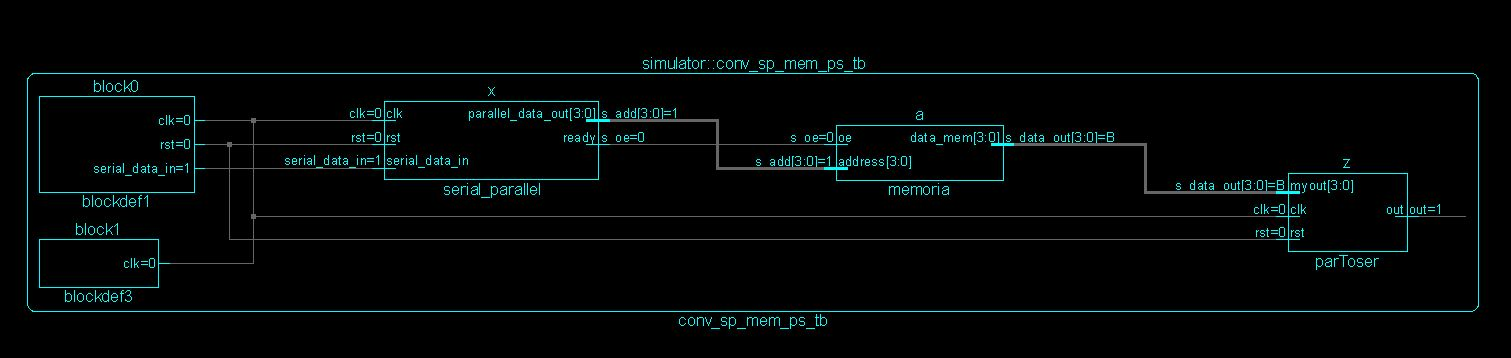
\includegraphics[width=\textwidth]{figuras/blocosdigitais.JPG}
  \caption{Bloco Digital Completo.}
  \label{bdc}
\end{figure}

Através de um arquivo \textit{testbench} foram adicionados estímulos conhecidos para realizar a simulação: A entrada 'rst' começa em nível lógico alto para que seja feita a iniciação e em seguida fica em nível lógico baixo pelo resto da simulação. Na entrada 'clk' é adicionado um clock simétrico com um período de 100ns. Finalmnente, na entrada serial do bloco foi adicionado uma sequência de valores lógicos para que se pudesse adquirir o endereço desejado na memória.

A figura \ref{sbdc} mostra o resultado da simulação. É possível observar que o funcionamento é conforme o esperado.A cada subida de clock, após a entrada 'rst' ir para nível lógico baixo, o contador interno é incrementado, e na quarta situação de subida de clock o sinal de controle 'oe' alcança nível lógico alto. Neste momento, o bloco de memória recebe o endereço do dado requisitado, palavra esta que estava sendo construída a cada subida de clock anteriormente (como pode ser visto no sinal s add[3:0]).

\begin{figure}[ht!]
  \centering
  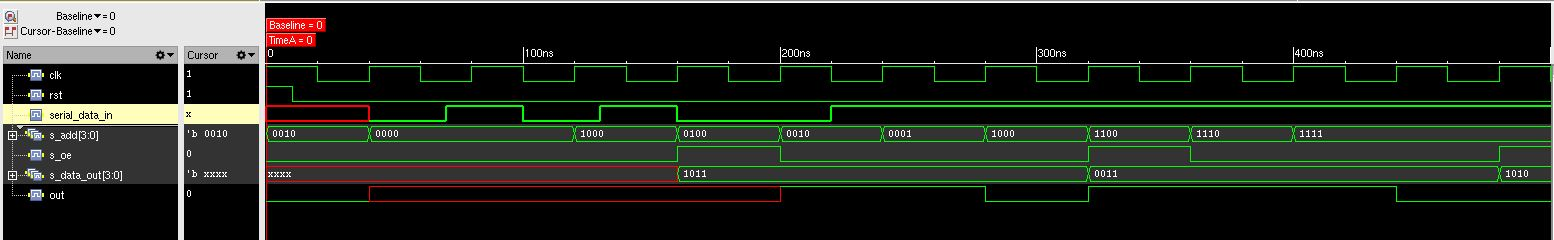
\includegraphics[width=\textwidth]{figuras/simbd.JPG}
  \caption{Simulação do Bloco Digital Completo.}
  \label{sbdc}
\end{figure}


\section{Simulação do Bloco Analógico}

Simulações realizadas em \cite{Marlon} demonstram que o bloco do demodulador funciona de forma satisfatória isoladamente. A modelagem em Verilog-AMS foi feita usando 3 sub-blocos: detector de envoltória, filtro de média e comparador com histerese. A Figura \ref{dem} mostra simulações do bloco demodulador realizadas em \cite{Marlon}, sendo possível observar as saídas intermediárias do detector de envoltória e do filtro de média.

\begin{figure}[ht!]
  \centering
  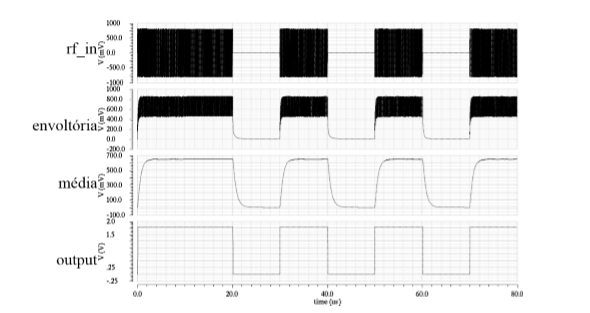
\includegraphics[width=\textwidth]{figuras/dem.PNG}
  \caption{Simulação do Demodulador ASK em Verilog-AMS\cite{Marlon}.}
  \label{dem}
\end{figure}

\section{Simulação Mista}